\documentclass[tikz,border=14pt]{standalone}
\usepackage[T1]{fontenc}
\usepackage{tgheros}
\usepackage{sfmath}
\usepackage{amsmath}
\usepackage{fontawesome5}
\usepackage{tikz}
\usetikzlibrary{arrows.meta,positioning,shapes.geometric,fit,backgrounds,calc}
\usepackage{xcolor}

\renewcommand{\familydefault}{\sfdefault}

% Harvard Crimson & ETH Zurich Academic Semantic Palette
\definecolor{harvardcrimson}{HTML}{A51C30}
\definecolor{ethdarkblue}{HTML}{1F407A}
\definecolor{ethblue}{HTML}{215CAF}
\definecolor{ethpetrol}{HTML}{007A87}
\definecolor{ethbronze}{HTML}{B87333}
\definecolor{ethpurple}{HTML}{5B4B8A}
\definecolor{ethslate}{HTML}{475569}
\definecolor{cardbg}{HTML}{F8FAFC}
\definecolor{cardborder}{HTML}{CBD5E1}
\definecolor{safeTeal}{HTML}{10B981}
\definecolor{faultCoral}{HTML}{DC2626}

\begin{document}
\begin{tikzpicture}[
  font=\sffamily,
  >=Stealth,
  layercard/.style={
    draw=faultCoral!70,
    fill=faultCoral!5,
    rounded corners=4pt,
    line width=0.9pt,
    text width=2.45in,
    inner sep=6pt,
    align=left
  },
  systemcard/.style={
    draw=ethdarkblue,
    fill=white,
    rounded corners=5pt,
    line width=1pt,
    text width=3.30in,
    inner sep=7pt,
    align=left
  },
  enforcercard/.style={
    draw=safeTeal,
    fill=safeTeal!8,
    rounded corners=5pt,
    line width=1.4pt,
    text width=3.30in,
    inner sep=8pt,
    align=left
  },
  faulttag/.style={
    font=\sffamily\bfseries\tiny,
    fill=white,
    draw=faultCoral!60,
    text=faultCoral,
    rounded corners=2pt,
    inner sep=2pt
  }
]

  % Top Title Banner
  \node[draw=ethdarkblue, fill=ethdarkblue!5, rounded corners=5pt, line width=1pt, text width=10.00in, inner sep=7pt, align=center] (title) at (5.00in, 0) {
    {\normalsize\bfseries\color{ethdarkblue}\faIcon{bomb}\;\; CROSS-LAYER SEEDED FAULT INJECTION ARCHITECTURE}\\[2pt]
    {\scriptsize\color{ethslate}Stress-Testing Every Architectural Layer to Verify Deterministic MCU Safety Containment}
  };

  % --- LEFT COLUMN: 4 FAULT INJECTION LAYERS ---
  \node[layercard, below=0.25in of title.south west, anchor=north west] (l1) {
    {\scriptsize\bfseries\color{faultCoral}\faIcon{video}\; LAYER 1: SENSORY \& TRANSDUCTION}\\[2pt]
    {\tiny\color{ethslate}
    $\bullet$ Dropped MIPI camera frames ($> 100\text{ ms}$)\\
    $\bullet$ Optical blinding glare / sudden lux drop\\
    $\bullet$ PTP IEEE-1588 clock skew ($> 5\text{ ms}$)\\
    $\bullet$ Depth map sensor dropout / lens mud
    }
  };

  \node[layercard, below=0.15in of l1] (l2) {
    {\scriptsize\bfseries\color{faultCoral}\faIcon{microchip}\; LAYER 2: COMPUTE, BUS \& MEMORY}\\[2pt]
    {\tiny\color{ethslate}
    $\bullet$ Linux kernel panic / thread crash\\
    $\bullet$ Synthetic DMA memory bus saturation\\
    $\bullet$ \texttt{malloc} allocation stalls \& page faults\\
    $\bullet$ SPI / CAN-FD CRC checksum corruption
    }
  };

  \node[layercard, below=0.15in of l2] (l3) {
    {\scriptsize\bfseries\color{faultCoral}\faIcon{brain}\; LAYER 3: MODEL \& ALGORITHMIC}\\[2pt]
    {\tiny\color{ethslate}
    $\bullet$ Hallucinated 3D bounding boxes\\
    $\bullet$ Out-of-workspace trajectory proposals\\
    $\bullet$ Discontinuous acceleration jumps\\
    $\bullet$ Adversarial visual perturbation patches
    }
  };

  \node[layercard, below=0.15in of l3] (l4) {
    {\scriptsize\bfseries\color{faultCoral}\faIcon{bolt}\; LAYER 4: ELECTRICAL \& PHYSICAL}\\[2pt]
    {\tiny\color{ethslate}
    $\bullet$ Motor driver over-temperature ($> 105^\circ\text{C}$)\\
    $\bullet$ Battery bus voltage sag / brownout ($< 10.5\text{ V}$)\\
    $\bullet$ Sudden external collision load torque\\
    $\bullet$ Encoder phase loss / line break
    }
  };

  % --- CENTER COLUMN: DUAL-BRAIN ARCHITECTURE ---
  \node[systemcard] (mpu) at (5.30in, -1.05in) {
    {\scriptsize\bfseries\color{ethbronze}\faIcon{server}\; APPLICATION PROCESSOR (Linux MPU $\cdot$ System 2/1.5)}\\[2pt]
    {\tiny\color{ethslate}
    $\bullet$ Runs Vision Transformers, Deliberation \& Action Chunking\\
    $\bullet$ Untrusted, stochastic, prone to crashes and latency tails\\
    $\bullet$ Emits candidate trajectory buffer $\mathbf{p}_t$ over shared IPC link
    }
  };

  \node[enforcercard, below=0.22in of mpu] (mcu) {
    {\small\bfseries\color{safeTeal}\faIcon{shield-alt}\; REAL-TIME SAFETY ENFORCER (MCU $\cdot$ System 1)}\\[3pt]
    {\scriptsize\color{ethslate}\raggedright
    \textbf{1. Control Barrier Function Invariant ($h(x) \ge 0$):}\\
    \hspace*{6pt}Projects candidate $\mathbf{p}_t$ onto forward invariant safe set $\mathcal{C}$\\[2pt]
    \textbf{2. Dynamic Stopping Clearance Check ($d_{\text{gap}} > d_{\text{stop}}$):}\\
    \hspace*{6pt}Vetoes proposals exceeding braking envelope\\[2pt]
    \textbf{3. Zero-Software Hardware Watchdog Monitor:}\\
    \hspace*{6pt}Trips Category 1 dynamic stop if MPU heartbeat $> 50\text{ ms}$
    }
  };

  \node[draw=ethdarkblue, fill=ethdarkblue!8, rounded corners=4pt, line width=1pt, text width=3.30in, inner sep=6pt, below=0.18in of mcu] (plant) {
    {\scriptsize\bfseries\color{ethdarkblue}\faIcon{cogs}\; PHYSICAL PLANT \& ACTUATION ($W_t \to W_{t+1}$)}\\[2pt]
    {\tiny\color{ethslate}
    $\bullet$ Closed-loop motor current loops $\cdot$ Mechanical brakes $\cdot$ Verified safe stop
    }
  };

  % Fault Injection Injection Arrows (clean orthogonal paths)
  \draw[->, line width=1.1pt, dashed, faultCoral] (l1.east) -- node[pos=0.45, above, faulttag] {\faIcon{syringe}\; Camera Drop} ++(0.95in, 0) |- (mpu.west);
  \draw[->, line width=1.1pt, dashed, faultCoral] (l2.east) -- node[pos=0.45, above, faulttag] {\faIcon{syringe}\; Kernel Panic} ++(0.70in, 0) |- ($(mpu.south west)!0.5!(mcu.north west)$);
  \draw[->, line width=1.1pt, dashed, faultCoral] (l3.east) -- node[pos=0.45, above, faulttag] {\faIcon{syringe}\; Hallucination} ++(0.95in, 0) |- (mcu.west);
  \draw[->, line width=1.1pt, dashed, faultCoral] (l4.east) -- node[pos=0.45, above, faulttag] {\faIcon{syringe}\; Voltage Sag} ++(0.95in, 0) |- (plant.west);

  % Safety Handoff Arrows
  \draw[->, line width=1.2pt, ethbronze, dashed] (mpu.south) -- node[midway, fill=white, draw=cardborder, rounded corners=2pt, font=\sffamily\bfseries\tiny, text=ethbronze] {Candidate $\mathbf{p}_t$} (mcu.north);
  \draw[->, line width=1.5pt, safeTeal] (mcu.south) -- node[midway, fill=white, draw=safeTeal, rounded corners=2pt, font=\sffamily\bfseries\tiny, text=safeTeal] {Permitted $\mathbf{u}_t$ / E-Stop} (plant.north);

  % RIGHT COLUMN: PASS CRITERIA CARD
  \node[draw=safeTeal, fill=white, rounded corners=5pt, line width=1.1pt, text width=2.15in, anchor=north west] at (7.65in, -0.65in) {
    {\scriptsize\bfseries\color{safeTeal}\faIcon{check-double}\; PASS CRITERION}\\[4pt]
    {\scriptsize\color{ethslate}\raggedright
    \textbf{100\% Containment Rate:}\\
    $\bullet$ Zero collisions ($d_{\text{gap}} > 0$)\\
    $\bullet$ Bounded stopping time\\
    $\bullet$ Controlled halt $< 50\text{ ms}$\\[6pt]
    \textbf{Zero Uncontained Escapes:}\\
    Any single uncontained fault trips a \textbf{REFUSE} release verdict.\\[6pt]
    \textbf{Hardware Watchdog:}\\
    Dedicated non-maskable timer operates \mbox{independently} of Linux OS.
    }
  };

\end{tikzpicture}
\end{document}
